\documentclass[10pt]{beamer}
\usepackage{amsmath, amsfonts, amssymb}
\usepackage{zju_simple}
\usepackage{algorithm, algorithmic, setspace}
\usepackage{array}
\usepackage{multicol}
\usepackage{caption}
\usepackage{hyperref}
\hypersetup{
    colorlinks=true,
    linkcolor=blue,
    filecolor=magenta,      
    urlcolor=cyan,
}

\usefonttheme{professionalfonts}

\setbeamertemplate{section in toc}[sections numbered]
\setbeamerfont{footline}{size=\fontsize{6}{8}\selectfont}
\setbeamertemplate{footnote}{%
  \usebeamercolor{footnote}\hbox to 0.8em{\hfil\insertfootnotemark}\insertfootnotetext\par%
}
\addtobeamertemplate{footnote}{}{\vspace{2.5ex}}

\makeatletter
\def\th@mystyle{%
    \normalfont % body font
    \setbeamercolor{block title example}{bg=orange,fg=white}
    \setbeamercolor{block body example}{bg=orange!20,fg=black}
    \def\inserttheoremblockenv{exampleblock}
  }
\makeatother
\theoremstyle{mystyle}

%-------------------------------------------------------------------------
\newcommand{\MyHref}[3][blue]{\href{#2}{\color{#1}{#3}}}%
%-------------------------------------------------------------------------
\def\bb#1{\mathbf{#1}}
\newcommand{\bs}{\boldsymbol}
\newcommand{\bst}{\boldsymbol\theta}
%-------------------------------------------------------------------------
\let\oldfootnotesize\footnotesize
\renewcommand{\footnoterule}{%
\kern -3pt
\hrule width \textwidth height 0pt
\kern 3pt
}
\renewcommand*{\footnotesize}{\oldfootnotesize\tiny}
\newcommand\blfootnote[1]{%
  \begingroup
  \renewcommand\thefootnote{}\footnote[frame]{#1}%
  \addtocounter{footnote}{-1}%
  \endgroup
}
%-------------------------------------------------------------------------
\definecolor{formula_body}{rgb}{1,0.898,0.8}
\definecolor{formula_title}{rgb}{1,0.5,0}
\newenvironment{formula}[1]{%
  \setbeamercolor{block body}{bg=formula_body}
  \setbeamercolor{block title}{bg=formula_title,fg=white}
  \begin{minipage}{0.95\linewidth}
	\begin{block}{#1}
}{\end{block}\end{minipage}}
%-------------------------------------------------------------------------
\definecolor{theo_body}{rgb}{0.9176, 0.9176, 0.9686}
\definecolor{theo_title}{rgb}{0.8392, 0.8392, 0.9373}
\makeatletter
\def\th@mystyle{%
    \normalfont % body font
	\setbeamercolor{blcok body example}{bg=theo_body}
	\setbeamercolor{block title example}{bg=theo_title}
    \def\inserttheoremblockenv{exampleblock}
  }
\makeatother
\theoremstyle{mystyle}
\newtheorem{customtheorem}{Theorem}
\newenvironment{theo}[1]{%
	\begin{minipage}{0.95\linewidth}
	\renewcommand\thecustomtheorem{#1}%
	\customtheorem
}{\endcustomtheorem\end{minipage}}
%-------------------------------------------------------------------------
\let\oldtableofcontents\tableofcontents
\renewcommand{\tableofcontents}[1][]{
	\begin{multicols}{2}
		\oldtableofcontents[#1]
	\end{multicols}
}
%############################################################################################
%%%%%%%%%%%%%%%%%%%%%%%%%%%%%%%%%%%%%%%%%%%%%%%%%%%%%%%%%%%%%%%%%%%%%%%%%%%%%%%%%%%%%%%%%%%%%
\title{Optimizers in Machine Learning}
\author{Jianwei Zhang}
\institute{ZJU CS}
\date{\today}

\begin{document}
{
	\setbeamertemplate{headline}{} 
	\frame{\titlepage}
}
\addtocounter{framenumber}{-1}

\section*{Outline}
\begin{frame}
	\frametitle{Outline}
	\tableofcontents
\end{frame}

%############################################################################################
%%%%%%%%%%%%%%%%%%%%%%%%%%%%%%%%%%%%%%%%%%%%%%%%%%%%%%%%%%%%%%%%%%%%%%%%%%%%%%%%%%%%%%%%%%%%%

\section{Gradient Descent}
\begin{frame}
	\frametitle{Gradient Descent}
	\begin{itemize}
		\item Find a local minimizer of a function $f(x)$
		\begin{theo}{}[First-Order Necessary Conditions]
			If $x^*$ is a local minimizer and $f$ is continuously differentiable in an open neighborhood of $x^*$, then $\nabla f(x^*)=0$.
		\end{theo}
	\end{itemize}

\begin{minipage}{0.465\linewidth}
	\begin{figure}
		\centering
		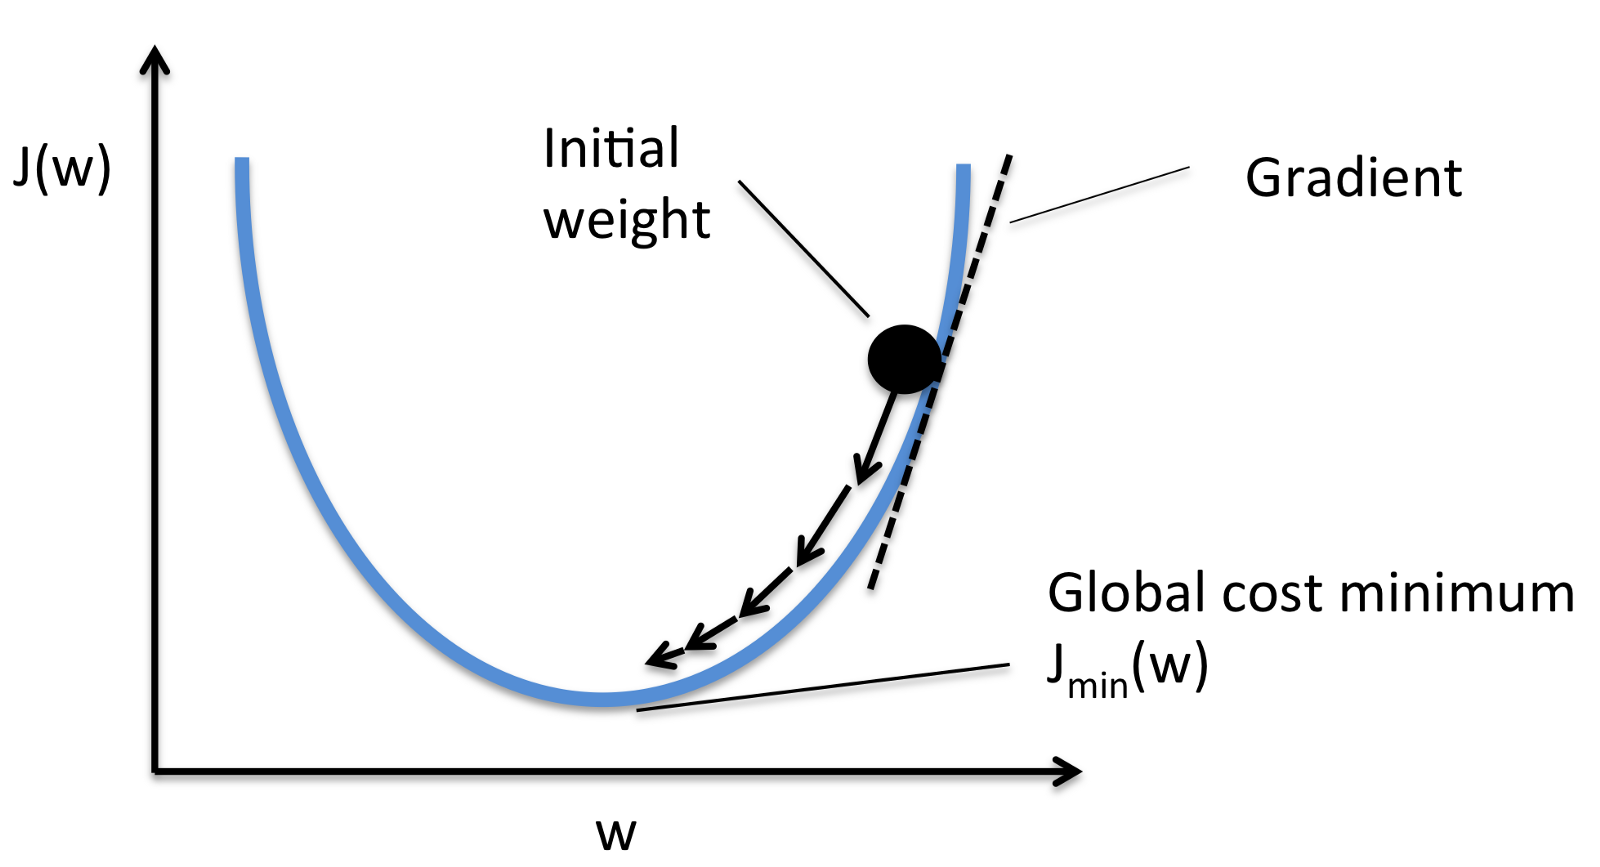
\includegraphics[width=0.95\linewidth]{images/fig-0.png}
	\end{figure}
\end{minipage}
\begin{minipage}{0.475\linewidth}
	\begin{figure}
		\centering
		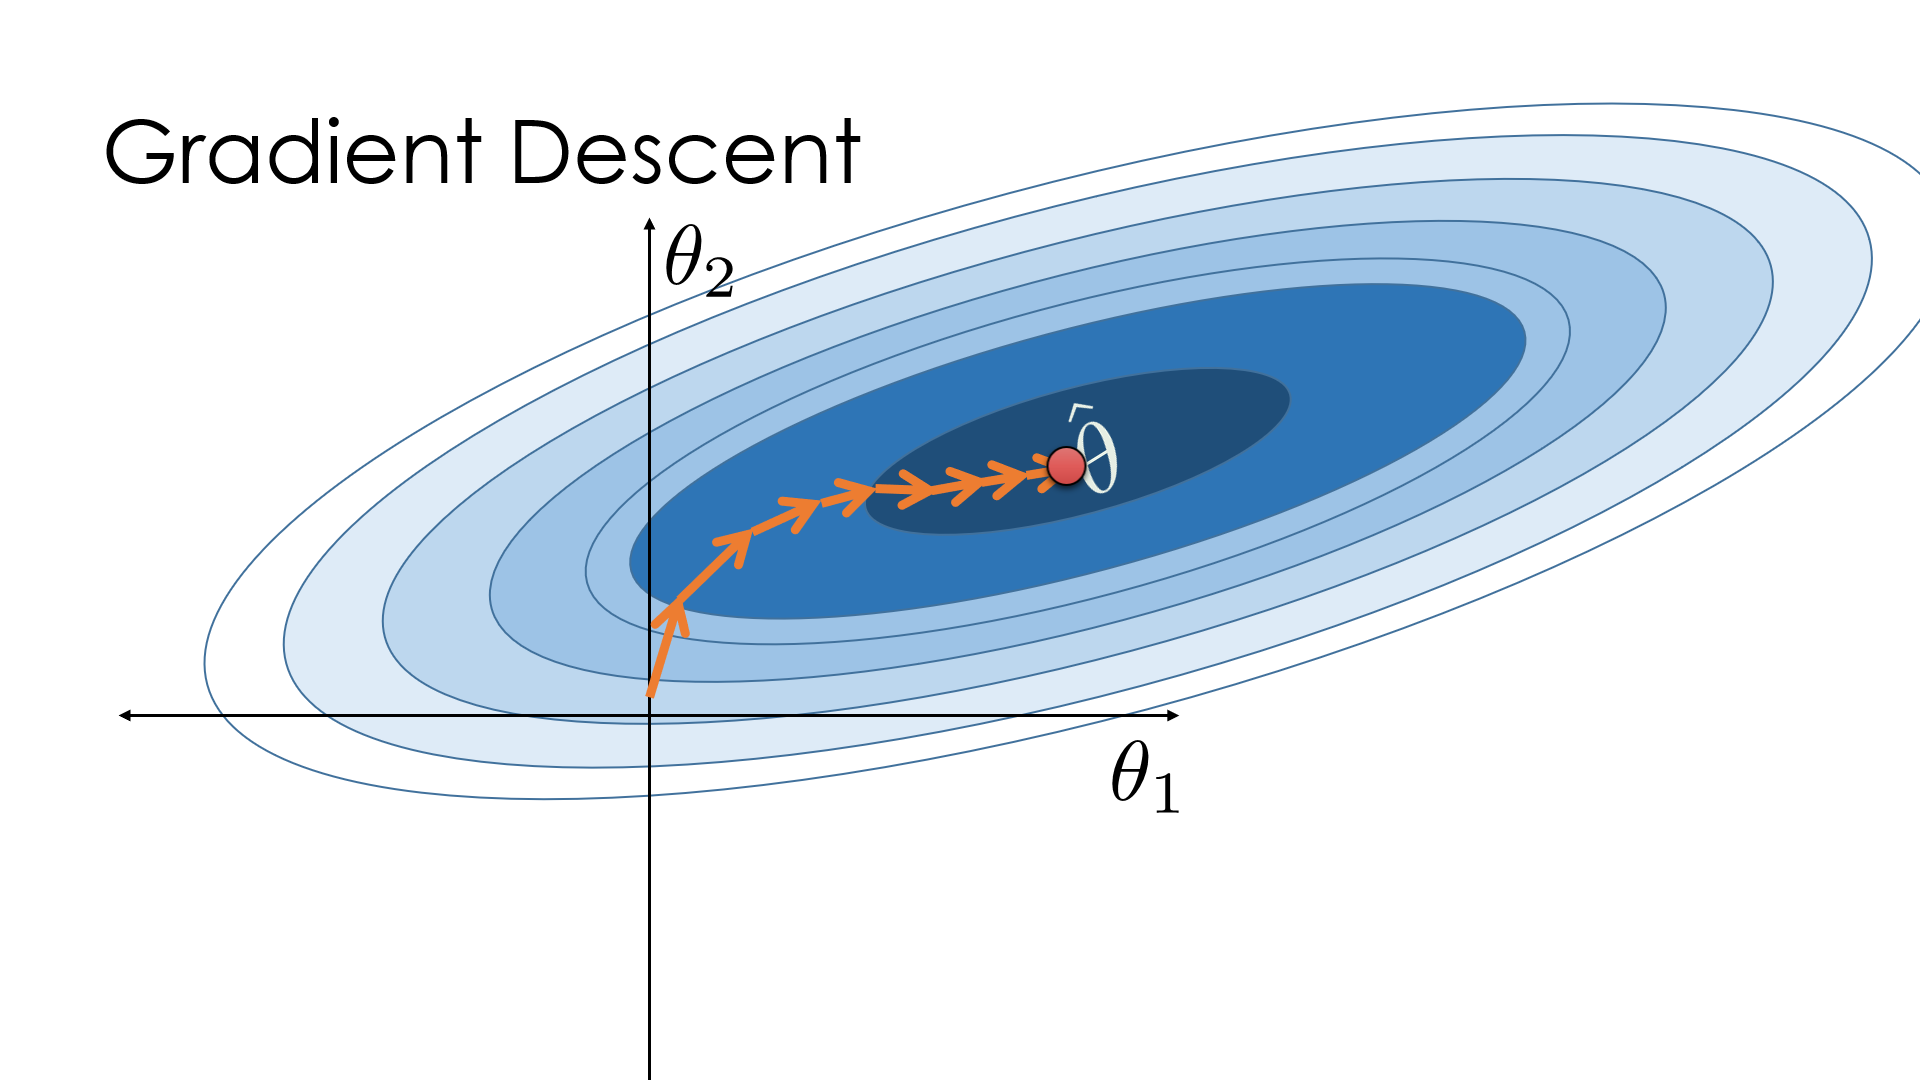
\includegraphics[width=0.95\linewidth]{images/fig-1.png}
	\end{figure}
\end{minipage}

\blfootnote{Nocedal J, Wright S. Numerical optimization[M]. Springer Science \& Business Media, 2006. Chapter 2}
\end{frame}

\begin{frame}
	\frametitle{Gradient Descent}
	\begin{algorithm}[H]
		\caption{Gradient Descent}
		\begin{algorithmic}[1]
		\REQUIRE Startint point $\bb{x}_0$
		\REQUIRE Step length $\gamma_t$
		\STATE Compute negative gradient direction $$\bb{p}_t=-\nabla f(\bb{x}_t)$$
		\STATE Move one step $$\bb{x}_{t+1}=\bb{x}_t+\gamma_t\bb{p}_t$$
		\STATE Loop line 1 and 2 until $\bb{p}_t\approx\bb{0}$
		\RETURN $\bb{x}_t$
		\end{algorithmic}
	\end{algorithm}
\end{frame}

\begin{frame}
	\frametitle{Gradient Descent}
	Machine Learning Model
	\begin{itemize}
		\item Model parameter $\bst$
		\item Dataset $\{\bb{z}_i\vert i=1,2,\cdots, n\}$
		\item Empirical error $f(\bb{z}_i\vert\bst)$, and $f$ is differentiable
		\item Goal $$\bst^*=\min_{\bst}\frac1{n}\sum_{i=1}^n f(\bb{z}_i\vert\bst)$$
	\end{itemize}
\end{frame}

\begin{frame}
	\frametitle{Gradient Descent}
	\begin{algorithm}[H]
		\caption{Gradient Descent in ML}
		\begin{algorithmic}[1]
		\REQUIRE Initial parameters $\bst$
		\REQUIRE Learning rate $\gamma_t$
		\STATE Compute negative gradient direction 
		\begin{equation}\label{eq:1}
			\bb{p}_t=-\frac1{n}\sum_{i=1}^n\nabla_{\bst}f(\bb{z}_i\vert\bst)
		\end{equation}
		\STATE Update parameters $$\bst\leftarrow\bst+\gamma_t\bb{p}_t$$
		\STATE Loop line 1 and 2 until $\bb{p}_t\approx\bb{0}$
		\RETURN $\bst$
		\end{algorithmic}
	\end{algorithm}
\end{frame}

%-------------------------------------------------------------------------
\section{Stochastic Gradient Descent}

\subsection{SGD}
\begin{frame}
	\frametitle{Stochastic Gradient Descent}
	\begin{itemize}
		\item It is hard to compute gradients of the empirical error in \eqref{eq:1} when we have a large-scale dataset. So we have {\bf stochastic gradient descent}:
		\begin{itemize}
			\item Estimate empirical error $E_n(f_{\bst})$ by a single randomly picked example $\bb z_t$ at step $t$ at each iteration: 
			\begin{equation}\label{eq:2}
				\bst\leftarrow\bst-\gamma_t\nabla_{\bst}f(\bb{z}_t\vert\bst)
			\end{equation}
			\item The stochastic process $\{\bst_t, t=1,2,\cdots\}$ depends on the examples randomly picked at each iteration.
			\item It is {\it hoped} that \eqref{eq:2} behaves like its expectation \eqref{eq:1} despite the noise introduced by this approximation.
			\item Convergence results usually require decreasing learning rate satisfying the conditions $\sum_t\gamma_t^2<\infty$ and $\sum_t\gamma_t=\infty$.
		\end{itemize}
	
	\end{itemize}
	\blfootnote{Bottou L. Large-scale machine learning with stochastic gradient descent[M]//Proceedings of COMPSTAT'2010. Physica-Verlag HD, 2010: 177-186.}
\end{frame}

\subsection{Average SGD}
\begin{frame}
	\frametitle{Average Stochastic Gradient Descent}
	\begin{itemize}
		\item {\bf Average Stochastic Gradient Descent (ASGD)} performs Normal SGD update and recursively computes the average $\overline{\bst}_t=\frac1{t}\sum_{i=1}^t\bst_i$:
		\begin{align}
			\bst_{t+1} &= \bst_t-\gamma_t\nabla_{\bst}f(\bb z_t\vert\bst), \\
			\overline{\bst}_{t+1} &= \frac{t}{t+1}\overline{\bst}_t + \frac1{t+1}\bst_{t+1}.
		\end{align}
		Notice that $\overline{\bst}$ is the desired parameter. Generally, ASGD might need a large amount of data to converge.
		\item A proper learning rate schedule used in ASGD: $$\gamma_t=\gamma_0(1+a\gamma_0t)^c,$$ with which we can takes a reasonable amount of data to reach its \href{https://en.wikipedia.org/wiki/Asymptotic_analysis}{asymptotic region}.
	\end{itemize}
	\blfootnote{Boris T. Polyak and Anatoli. B. Juditsky. Acceleration of stochastic approximation by averaging.
	Automation and Remote Control, 30(4):838–855, 1992.\\Xu W. Towards optimal one pass large scale learning with averaged stochastic gradient descent[J]. arXiv preprint arXiv:1107.2490, 2011.}
\end{frame}

\subsection{Batch SGD}
\begin{frame}
	\frametitle{Batch Stochastic Gradient Descent}
	\begin{itemize}
		\item Batch SGD is a compromise for estimating gradients.
	\end{itemize}
	\begin{table}
		{\renewcommand\arraystretch{1.4}
		\begin{tabular}{cll}
			\hline
			\bf Optimizer & \bf Use data & \bf Gradients \\ \hline
			GD & all data & $\frac1{n}\sum_{i=1}^n\nabla f(\bb z_i)$ \\
			SGD & single data per step & $\nabla f(\bb z_t)$ \\
			Batch SGD & a batch of data & $\frac1{m}\sum_{i=1}^m\nabla f(\bb z_i),\;m < n$ \\
			Mini-Batch SGD & a mini-batch of data & $\frac1{m}\sum_{i=1}^m\nabla f(\bb z_i),\;m\ll n$ \\ \hline
		\end{tabular}}
		\caption{GD and variants}
	\end{table}
\end{frame}

\begin{frame}
	\frametitle{Batch Stochastic Gradient Descent}
	\begin{itemize}
		\item Although batch GD has better performance in the figure below, a huge amount of non-convex functions will make (large) batch GD perform poorly.
	\end{itemize}
	\begin{figure}[H]
		\centering
		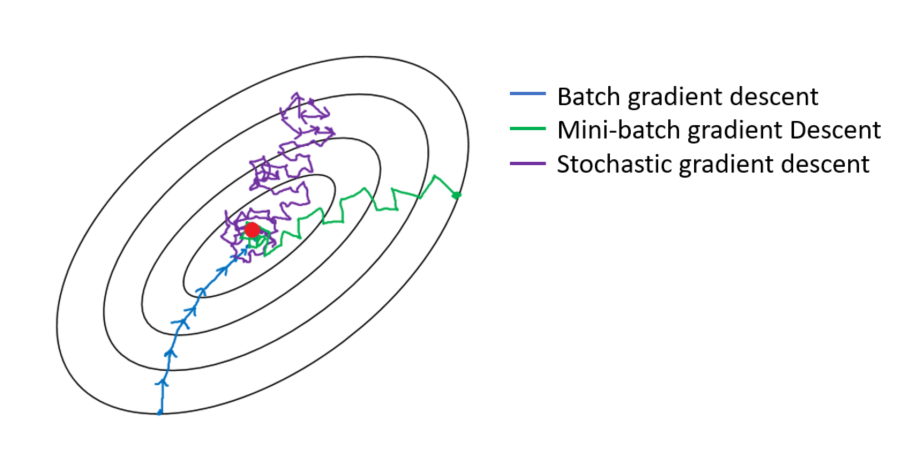
\includegraphics[width=0.8\linewidth]{images/fig-2.png}
	\end{figure}
\end{frame}

\subsection{Challenges}
\begin{frame}
	\frametitle{Influence on learning rate}
	\centering
		\begin{tabular}{m{4cm} m{12cm}}
			learning rate $0.0005$ &
			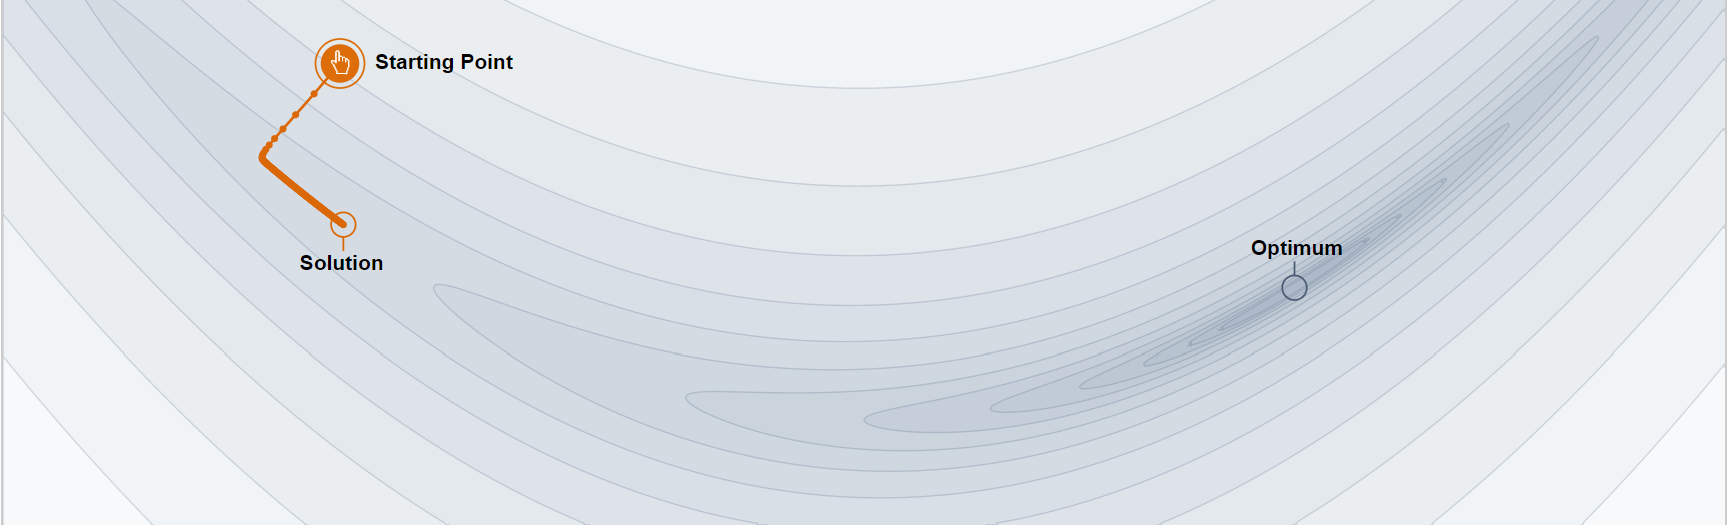
\includegraphics[width=0.45\linewidth]{images/lr-0005.png} \\
			learning rate $0.003$ &
			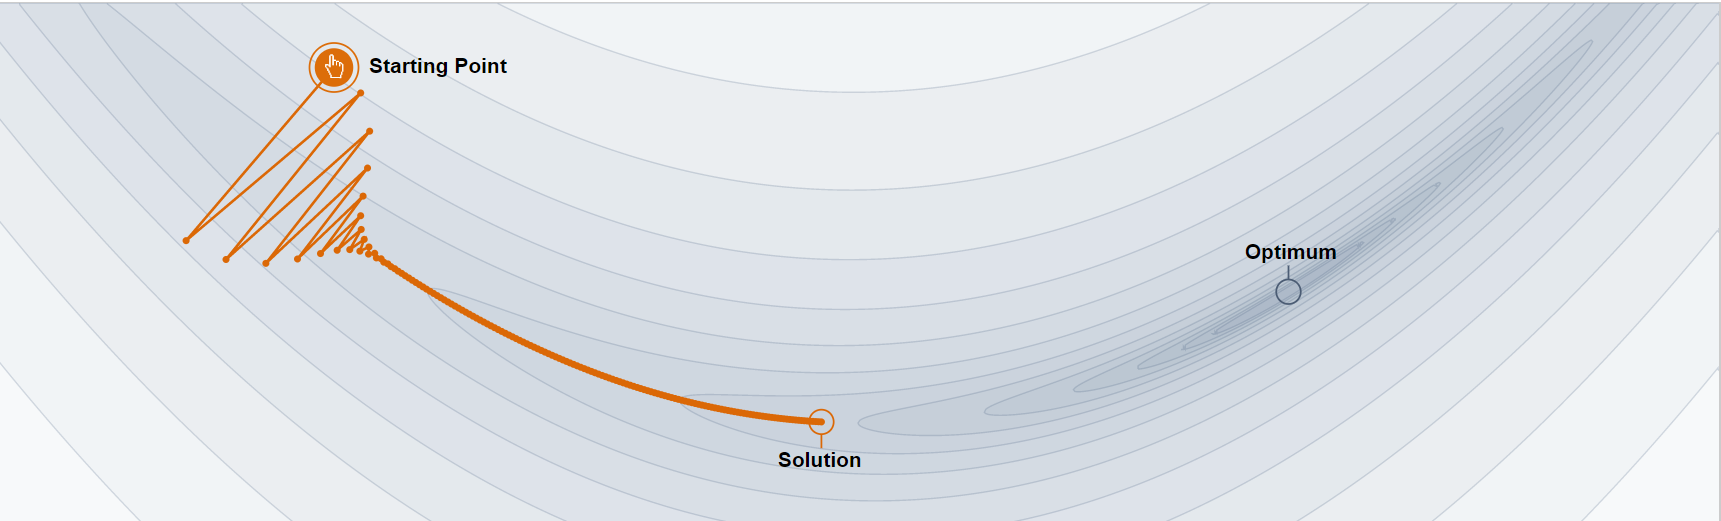
\includegraphics[width=0.45\linewidth]{images/lr-003.png} \\
			learning rate $0.004$ &
			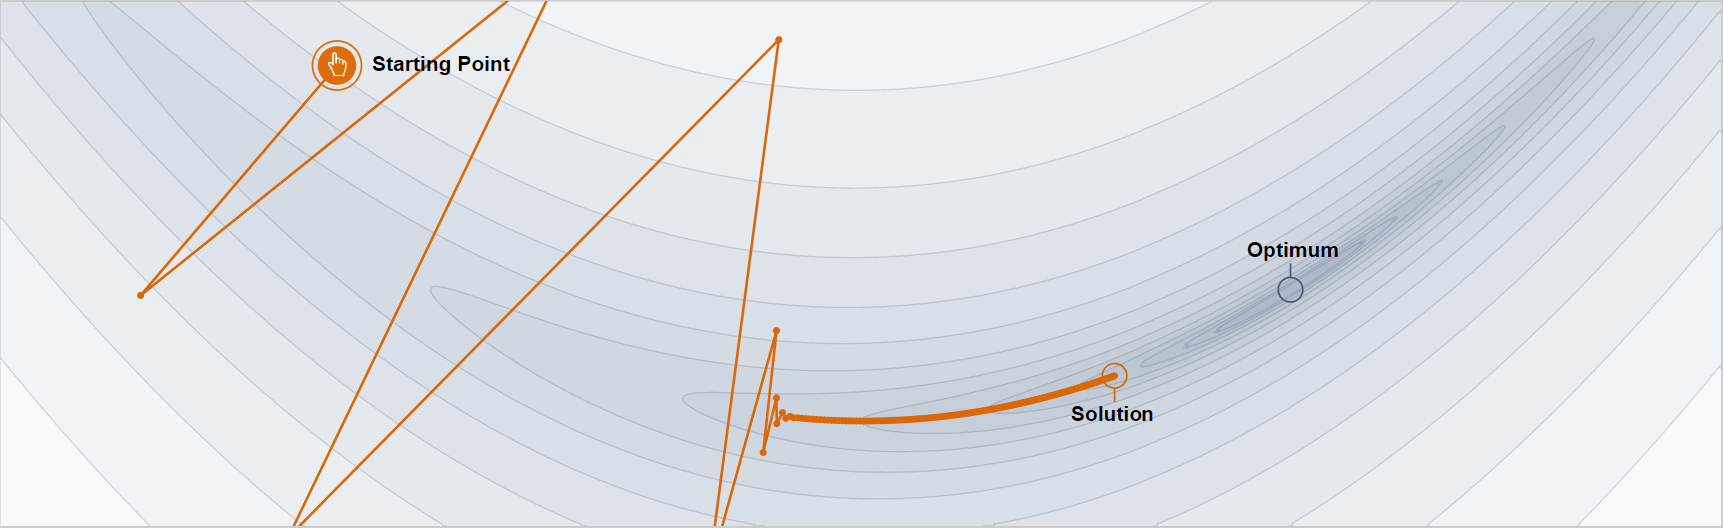
\includegraphics[width=0.45\linewidth]{images/lr-004.png} \\
			learning rate $0.005$ &
			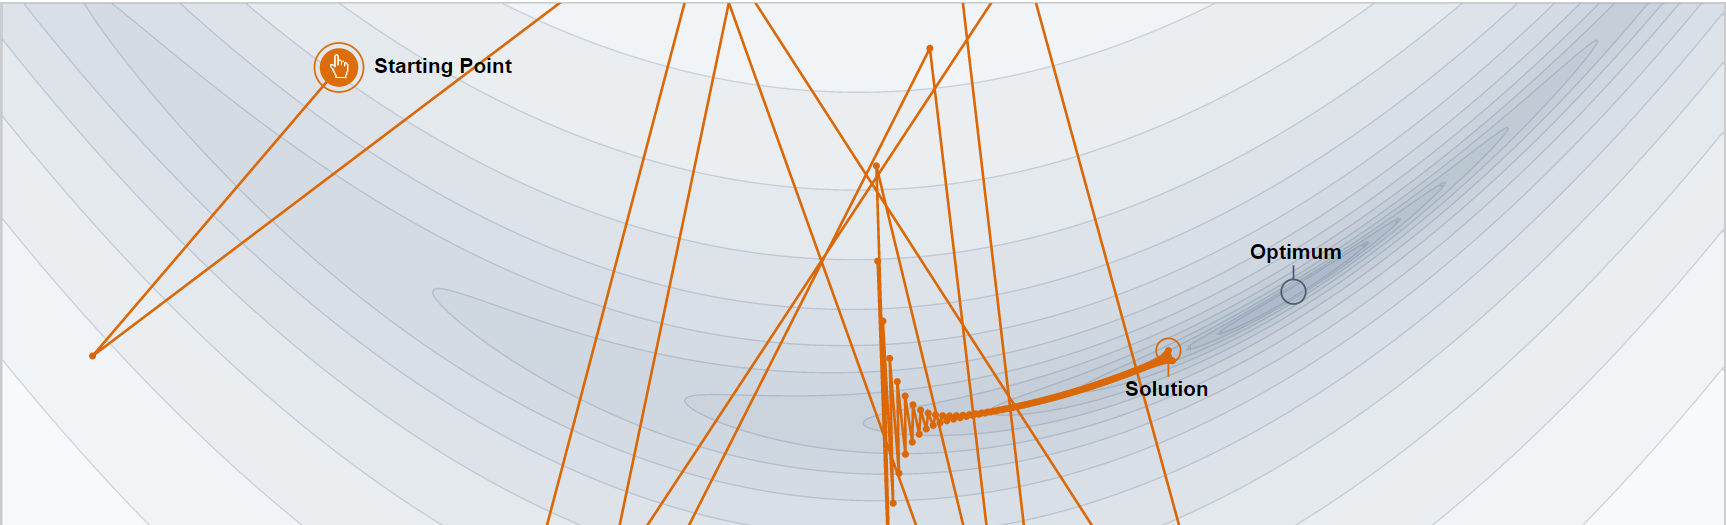
\includegraphics[width=0.45\linewidth]{images/lr-005.png} \\
		\end{tabular}
	\blfootnote{Figure: Why Momentum Really Works (\url{https://distill.pub/2017/momentum/})}
\end{frame}

\begin{frame}
	\frametitle{Challenges in SGD}
	\begin{itemize}
		\item Choose a proper learning rate is difficult.
		\item One learning rate schedule is unable to adapt to various datasets.
		\item Applying the same learning rate to all the parameters may not be the best.
		\item Object function is highly non-convex for neural networks, which means lost of local minima.
		\item Second-order optimization methods such as Newton's method are not suitable for deep learning. Because Hessian matrix is hard to compute.
	\end{itemize}
	\blfootnote{Ruder S. An overview of gradient descent optimization algorithms[J]. arXiv preprint arXiv:1609.04747, 2016.}
\end{frame}

%-------------------------------------------------------------------------
\section{Momentum and Nesterov}

\subsection{Exponentially Weighted Average}
\begin{frame}
	\frametitle{Exponentially Weighted Average}
	\begin{itemize}
		\item Samples from cosine function with Gaussian noise
	\end{itemize}
	\begin{figure}[H]
		\centering
		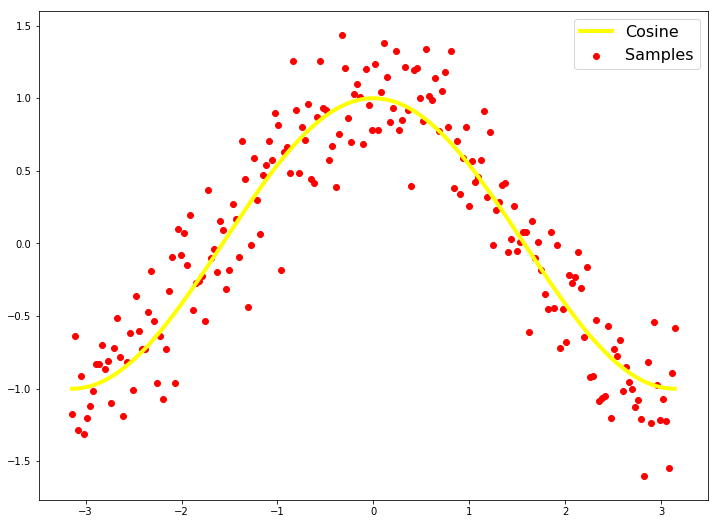
\includegraphics[width=0.5\linewidth]{images/fig-3.png}
	\end{figure}
\end{frame}

\begin{frame}
	\frametitle{Exponentially Weighted Average}
	\begin{itemize}
		\item We want some kind of 'moving' average which would 'denoise' the data and bring it closer to original function.
		\item Exponentially weighted averages define a new sequence 
	\end{itemize}
	\begin{figure}[H]
		\centering
		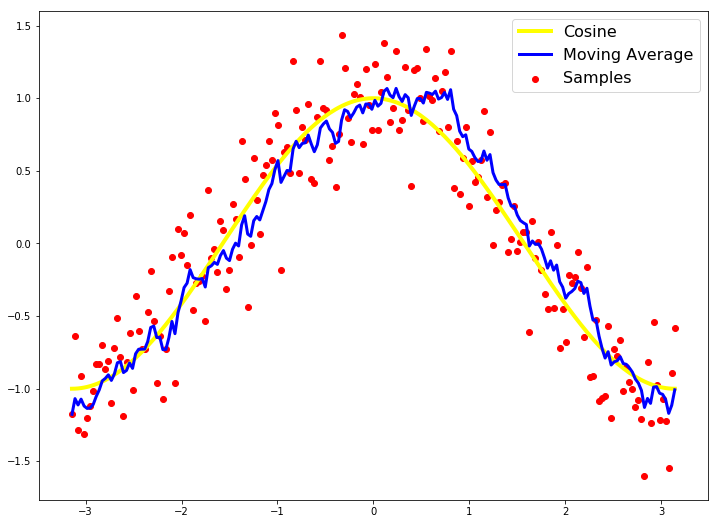
\includegraphics[width=0.5\linewidth]{images/fig-4.png}
	\end{figure}
\end{frame}

\begin{frame}
	\frametitle{Exponentially Weighted Average}
	\begin{itemize}
		\item Exponentially weighted average formula:
		\begin{equation}
			\bb m_t = \beta\bb m_{t-1} + (1-\beta)\hat{\bb m}_t,
		\end{equation}
		where $\{\bb m_t, t=1,2,\cdots\}$ is a new moving-averaged sequence. 
		\item Larger $\beta$ will give smoother sequences but cause more seriously 'decay'.
	\end{itemize}
	
	\begin{figure}[H]
		\centering
		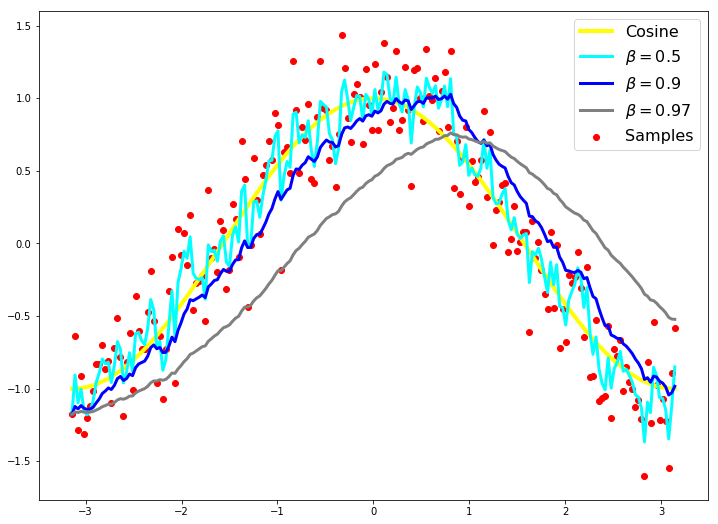
\includegraphics[width=0.5\linewidth]{images/fig-5.png}
	\end{figure}
\end{frame}

\subsection{Momentum SGD}

\begin{frame}
	\frametitle{SGD with Momentum}
	\begin{itemize}
		\item SGD has trouble navigating ravines(narrow valley), i.e. areas where the surface curves much more steeply in one dimension than in another, which are common around local optima. 
		\item The system will oscillate back and forth in the direction of short axis and move very slowly along the long axis of the valley.
		\item How to accelerate SGD? Momentum!
	\end{itemize}

	\begin{figure}[H]
		\centering
		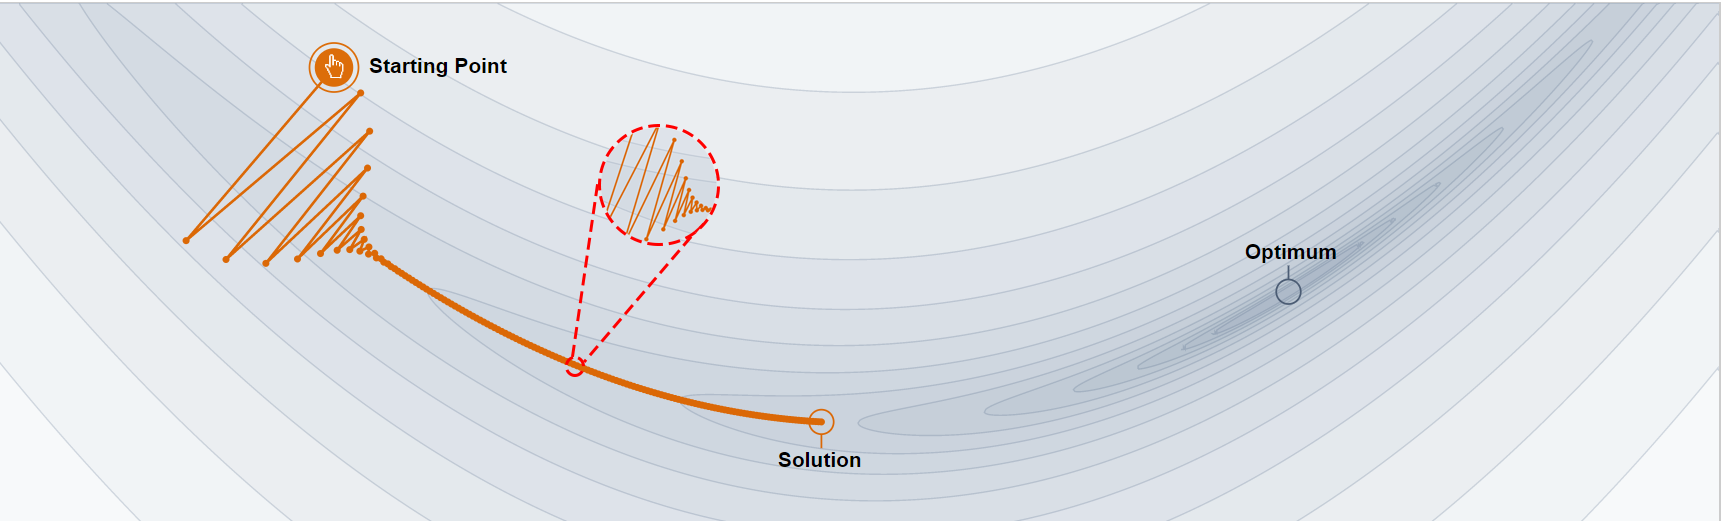
\includegraphics[width=0.8\linewidth]{images/oscillates.png}
		\caption{SGD without momentum, learning rate 0.003}
	\end{figure}
	\blfootnote{Figure: Why Momentum Really Works (\url{https://distill.pub/2017/momentum/})}
\end{frame}

\begin{frame}
	\frametitle{SGD with Momentum}
	\begin{itemize}
		\item Recall exponentially weighted average: 
		$$ \bb m_t = \beta\bb m_{t-1} + (1-\beta)\hat{\bb m}_t. $$
		\item Remove $1-\beta$ and let $\hat{\bb m}_t=\gamma\nabla_{\bst}f(\bst_t)$. Then we get 
		\begin{formula}{Momentum SGD}
			\begin{align}
				\bb m_t &= \beta\bb m_{t-1} + \gamma\nabla_{\bst}f(\bst_t), \quad 0<\beta<1 \\
				\bst_{t+1} &= \bst_t - \bb m_t
			\end{align}	
		\end{formula} 
		\item Usually momentum parameter $\beta$ is set to $0.9$ or $0.99$ that is close to $1$.
	\end{itemize}
\end{frame}

\begin{frame}
	\frametitle{SGD with Momentum}
	\begin{itemize}
		\item The modification of the parameters $\bst$ at the current times step depends on both the current gradient $\nabla_{\bst}f(\bst_t)$ and the parameters change $\bb m_t$ of the previous step. 
	\end{itemize}

	\begin{figure}[H]
		\centering
		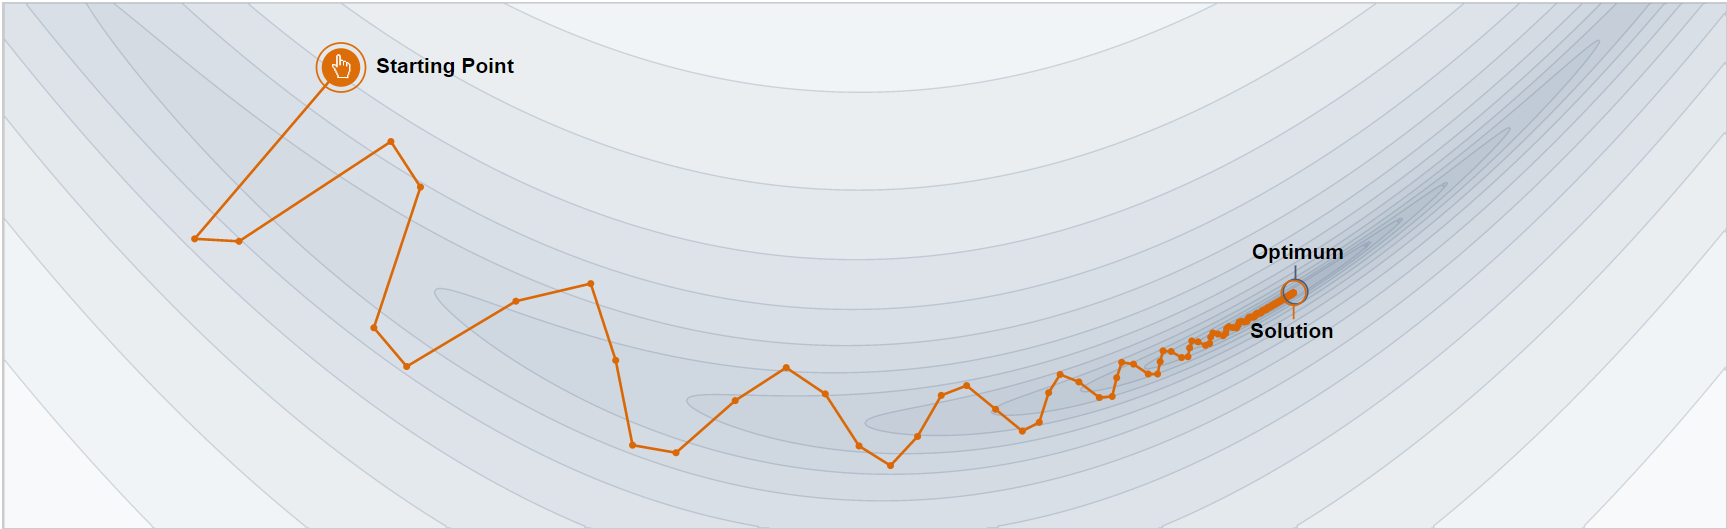
\includegraphics[width=0.8\linewidth]{images/mmt-85.png}
		\caption{SGD with momentum 0.85, learning rate 0.003}
	\end{figure}
	
	\blfootnote{Qian N. On the momentum term in gradient descent learning algorithms[J]. Neural networks, 1999, 12(1): 145-151.\\
	Figure: Why Momentum Really Works (\url{https://distill.pub/2017/momentum/})}
\end{frame}

\subsection{Nesterov SGD}

\begin{frame}
	\frametitle{Nesterov Accelerated Gradient}
	\begin{minipage}{0.73\linewidth}
		\begin{itemize}
			\item We will use momentum term $\beta\bb m_t$ to move parameter $\bst$. So computing a "look-ahead" $\bst-\beta\bb m_t$ will give us an approximation of the next position of the parameters, which we can use to estimate gradients.
		\end{itemize}
	\end{minipage}
	\begin{minipage}{0.25\linewidth}
		\begin{flushright}
			\begin{figure}[H]
				\centering
				
\includegraphics[width=\linewidth]{images/Yurii_Nesterov.png}
				\caption*{Yurii Nesterov}
			\end{figure}	
		\end{flushright}
	\end{minipage}
	
	\begin{itemize}
		\item We slightly adjust the formulas of Momentum SGD to get NAG:
		\begin{minipage}{0.95\linewidth}
			\begin{formula}{Nesterov accelerated gradient (NAG)}
				\begin{align}
					\bb m_t &= \beta\bb m_{t-1} + \gamma\nabla_{\bst}f(\bst_t-\beta\bb m_{t-1}),\quad 0<\beta<1 \\
					\bst_{t+1} &= \bst_t - \bb m_t
				\end{align}	
			\end{formula}
		\end{minipage}
	\end{itemize}
	
	\blfootnote{Nesterov Y. A method for unconstrained convex minimization problem with the rate of convergence O ($1/k^2$)[C]//Doklady AN USSR. 1983, 269: 543-547.}
\end{frame}

\begin{frame}
	\frametitle{Nesterov Accelerated Gradient}
	\begin{figure}[H]
		\centering
		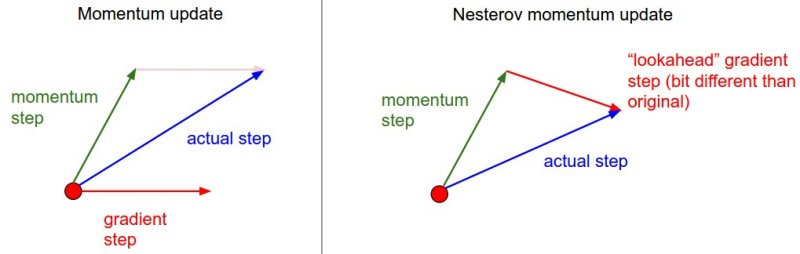
\includegraphics[width=0.8\linewidth]{images/fig-nesterov.jpeg}
		\caption{Momentum vs. Nesterov momentum}
	\end{figure}

	\blfootnote{CS231n Convolutional Neural Networks for Visual Recognition(\url{http://cs231n.github.io/neural-networks-3/\#sgd})}
\end{frame}

%-------------------------------------------------------------------------
\section{Adaptive Learning Rate}

\subsection{AdaGrad}
\begin{frame}
	\frametitle{AdaGrad}
	\begin{itemize}
		\item {\bf Adaptive gradient (AdaGrad)} adapts the learning rate to the parameters, performing larger updates for infrequent and smaller updates for frequent parameters.
		\begin{formula}{Adaptive gradient (AdaGrad)}
			\begin{equation}
				\bst_{t+1} = \bst_t - \frac{\gamma}{\sqrt{G_t+\epsilon}}\odot\nabla_{\bst}f(\bst_t),
			\end{equation}
			where $\odot$ is element-wise product, $\epsilon$ is a small number to prevent dividing by zero and $G_t\in\mathbb{R}^{d\times d}$ is a diagonal matrix where each diagonal element $(i, i)$ is the sum of the squares of the gradients w.r.t. $\bst^{(i)}$ up to time step $t$:
			$$
			G_t^{(i, i)} = \sum_{\tau=1}^t\nabla_{\bst}f(\bst_{\tau})^2
			$$
		\end{formula}
	\end{itemize}
	\blfootnote{Duchi J, Hazan E, Singer Y. Adaptive subgradient methods for online learning and stochastic optimization[J]. Journal of Machine Learning Research, 2011, 12(Jul): 2121-2159.}
\end{frame}

\begin{frame}
	\frametitle{AdaGrad}
	\begin{itemize}
		\item Advantages
		\begin{itemize}
			\item It is well suited for sparse data.
			\item It basically eliminates the need to tune the learning rate.
		\end{itemize}
		\item Disadvantages
		\begin{itemize}
			\item It is sensitive to the initial gradients. Large initial gradients result in lower learning rate and make training slower.
			\item Due to the continual accumulation of squared gradients in the denominator, the learning rate will continue to decrease throughout training, eventually decreasing to zero and stop training.
		\end{itemize}
	\end{itemize}

	\blfootnote{Ruder S. An overview of gradient descent optimization algorithms[J]. arXiv preprint arXiv:1609.04747, 2016.}
\end{frame}

\def\tt{\mathbb{E}}
\def\ttr{\text{RMS}}
\subsection{AdaDelta}
\begin{frame}
	\frametitle{AdaDelta}
	\begin{itemize}
		\item {\bf AdaDelta} is an extension of AdaGrad for reducing its aggressive, monotonically decreasing learning rate. A natural idea is to restrict the accumulation window of the squared gradients. However, instead of storing a series of gradients which is not an efficient choice, AdaDelta use a exponentially weighted average($\mathbb{E}$) of the square gradients:
		\begin{equation}
			\tt[\nabla_{\bst}f(\bst)^2]_t=\rho \tt[\nabla_{\bst}f(\bst)^2]_{t-1} + (1-\rho)\nabla_{\bst}f(\bst_t)^2.
		\end{equation}
		\item Denote $\ttr[\nabla_{\bst}f(\bst)]_t$ ({\bf R}oot {\bf M}ean {\bf S}quare) the square root of $\tt$:
		\begin{equation}
			\ttr[\nabla_{\bst}f(\bst)]_t = \sqrt{\tt[\nabla_{\bst}f(\bst)^2]_t +\epsilon}.
		\end{equation}
		\item But actually RMS represents \underline{Root Exponentially Weighted Average Square} here.
	\end{itemize}
	\blfootnote{Zeiler, Matthew D. 2012. “ADADELTA: An Adaptive Learning Rate Method.” ArXiv:1212.5701 [Cs], December. http://arxiv.org/abs/1212.5701.}
\end{frame}

\begin{frame}
	\frametitle{AdaDelta}
	\begin{itemize}
		\item Then we get parameter update:
		\begin{formula}{AdaDelta (Primary)}
			\begin{equation}\label{adadelta:1}
				\bst_{t+1} = \bst_t - \frac{\gamma}{\ttr[\nabla_{\bst}f(\bst)]_t}\odot\nabla_{\bst}f(\bst_t),
			\end{equation}
		\end{formula}
		\vspace{3mm}
		\item Notice that if the optimization problem(such as a physical problem) has some hypothetical units, then the update formula above will lead to wrong units(comparing to SGD, here exists an extra unit of gradients in denominator). So as to AdaGrad. 
	\end{itemize}
\end{frame}

\begin{frame}
	\frametitle{AdaDelta}
	\begin{itemize}
		\item Considering the units of SGD:
		\begin{equation}\label{adadelta:2}
			\text{units of}~\Delta\bst\propto\boxed{\text{units of}~\nabla_{\bst}f(\bst)\propto\frac{\partial f}{\partial\bst}}\propto\frac1{\text{units of}~\bst},
		\end{equation}
		assuming the cost function $f$ is unitless. 
		\item The SGD method will result in wrong units, while the second order methods such as Newton's method using Hessian information $H$ do have the correct units for the parameter update:
		\begin{equation}\label{adadelta:3}
			\Delta\bst\propto H^{-1}\nabla_{\bst}f(\bst)\propto\boxed{\frac{\frac{\partial f}{\partial\bst}}{\frac{\partial^2f}{\partial\bst^2}}\propto\text{units of}~\bst}.
		\end{equation}
		\item We rearrange Newton's method(assuming a diagonal Hessian) for the inverse of the second derivative to determine the quantities involved:
		\begin{equation}\label{adadelta:4}
			\Delta\bst=\frac{\frac{\partial f}{\partial\bst}}{\frac{\partial^2f}{\partial\bst^2}}\Rightarrow\boxed{\frac1{\frac{\partial^2f}{\partial\bst^2}}=\frac{\Delta\bst}{\frac{\partial f}{\partial\bst}}}.
		\end{equation}
	\end{itemize} 
\end{frame}

\begin{frame}
	\frametitle{AdaDelta}
	\begin{itemize}
		\item Use equation\eqref{adadelta:1} and boxed part of \eqref{adadelta:2},\eqref{adadelta:3}, we can know that unit of $\frac{\Delta\bst}{\frac{\partial f}{\partial\bst}}$ in equation \eqref{adadelta:4} is correct. So after applying some transformation, $\frac{\Delta\bst}{\frac{\partial f}{\partial\bst}}$ will be a proper substitute of $\frac{\gamma}{\ttr[\nabla_{\bst}f(\bst)]_t}$. 
		\item In denominator, $\frac{\partial f}{\partial\bst}$ is related to $\ttr[\nabla_{\bst}f(\bst)]_t$, so in numerator, we can similarly replace $\gamma$ with $\ttr[\Delta\bst]_t$. But we still do not have $\Delta\bst_t$, so we use a delayed version $\ttr[\Delta\bst]_{t-1}$. 
		\item Finally we have final AdaDelta algorithm
		\begin{formula}{AdaDelta (Final)}
			\begin{equation}
				\bst_{t+1} = \bst_t - \frac{\ttr[\Delta\bst]_{t-1}}{\ttr[\nabla_{\bst}f(\bst)]_t}\odot\nabla_{\bst}f(\bst_t),
			\end{equation}
		\end{formula}
	\end{itemize}
\end{frame}

\def\ggg{\nabla_{\bst}f(\bst)}
\def\ggt{\nabla_{\bst}f(\bst_t)}
\begin{frame}
	\frametitle{AdaDelta}
	\begin{algorithm}[H]
		\setstretch{1.3}
		\caption{AdaDelta}
		\begin{algorithmic}[1]
		\REQUIRE Decay rate $\rho$, Constant $\epsilon$
		\REQUIRE Initial parameter $\bst_0$
		\STATE Initialize accumulation variables $\tt[\ggg^2]_0=0, \tt[\Delta\bst^2]_0=0$
		\FOR{$t=1:T$ Loop over \# of updates}
		\STATE Compute Gradiet: $\ggt$
		\STATE Accumulate Gradient: $\tt[\ggg^2]_t=\rho\tt[\ggg^2]_{t-1}+(1-\rho)\ggt^2$
		\STATE Compute Update: $(\Delta\bst)^2_t=-\frac{\ttr[\Delta\bst]_{t-1}}{\ttr[\ggg]_t}\ggt$
		\STATE Accumulate Updates: $\tt[(\Delta\bst)^2]_t=\rho\tt[(\Delta\bst)^2]_{t-1}+(1-\rho)(\Delta\bst_t)^2$
		\STATE Apply Update: $\bst_{t+1}=\bst_t+\Delta\bst_t$
		\ENDFOR
		\end{algorithmic}
	\end{algorithm}
\end{frame}

\subsection{RMSProp}
\begin{frame}
	\frametitle{RMSProp}
	\begin{itemize}
		\item {\bf RMSProp}, proposed by Geoffery Hinton, is just the primary version of AdaDelta.
		\begin{formula}{RMSProp}
			\begin{equation}
				\bst_{t+1} = \bst_t - \frac{\gamma}{\ttr[\nabla_{\bst}f(\bst)]_t}\odot\nabla_{\bst}f(\bst_t),
			\end{equation}
		\end{formula}
		\item A typical choice of $\rho$ in $RMSProp$ is $0.9$.
	\end{itemize}

	\blfootnote{\MyHref[black]{http://www.cs.toronto.edu/~tijmen/csc321/slides/lecture_slides_lec6.pdf}{http://www.cs.toronto.edu/\~{}tijmen/csc321/slides/lecture\_slides\_lec6.pdf}}
\end{frame}


%-------------------------------------------------------------------------
\section{Adaptive Momentum}
\subsection{Adam}
\begin{frame}
	\frametitle{Adaptive Momentum, Adam}
	\begin{itemize}
		\item Inspired by AdaDelta storing exponentially weighted average of previous squared gradients(denote $\bb m_t$), {\bf Adaptive Momentum(Adam)} Estimation also keeps an exponentially weighted average of previous gradients(denote $\bb v_t$), similar to momentum:
		\begin{align}
			\bb m_t &= \beta_1\bb m_{t-1}+(1-\beta_1)\nabla_{\bst}f(\bst_t) \\
			\bb v_t &= \beta_2\bb v_{t-1}+(1-\beta_2)\nabla_{\bst}f(\bst_t)^2 
		\end{align}
		where $\bb m_t$ and $\bb v_t$ can also be regarded as the first moment(the mean) and the second moment(the uncentered variance) of the gradients, respectively. 
		\item $\beta_1$ and $\beta_2$ are close to $1$ just like Momentum, and RMSProp.
		\item Notice that if we initialize $\bb m_0=\bb0$ and $\bb v_0=\bb0$, then the gradients are biased towards zero, especially in initial steps.
	\end{itemize}
	
	\blfootnote{Kingma, Diederik P., and Jimmy Ba. 2014. “Adam: A Method for Stochastic Optimization.” ArXiv:1412.6980 [Cs], December. http://arxiv.org/abs/1412.6980.}
\end{frame}

\begin{frame}
	\frametitle{Adaptive Momentum, Adam}
	\begin{itemize}
		\item We need the algorithm have larger moments at the beginning of training to counteract the biases mentioned above:
		\begin{align}\label{adam:mhat}
			&\hat{\bb m}_t=\frac{\bb m_t}{1 - \beta_1^t}, \\ \label{adam:vhat}
			&\hat{\bb v}_t=\frac{\bb v_t}{1 - \beta_2^t}.
		\end{align}
		And we give a brief derivation of equation \eqref{adam:mhat} and \eqref{adam:vhat} in next slide.
		\item Finally we get Adam update rule:
		\begin{equation}
			\bst_{t+1}=\bst_t-\frac{\gamma}{\sqrt{\hat{\bb v}_t}+\epsilon}\hat{\bb m}_t.
		\end{equation}
	\end{itemize}
\end{frame}

\begin{frame}
	\frametitle{Proof of Bias-Correction*}
	\begin{itemize}
		\item Let $\bb g=\nabla_{\bst}f(\bst)$. For the exponentially weighted average, we have
		\begin{equation}\label{adam:sum}
			\bb v_t = \beta_2\bb v_{t-1}+(1-\beta_2)g_t^2 = (1-\beta_2)\sum_{i=1}^t\beta_2^{t-i}\bb g^2.
		\end{equation}
		We wish to know how $\mathbb{E}[\bb v_t]$, the expected value of the exponentially weighted average at timestep $t$, relates to the true second order moment $\mathbb{E}[\bb g_t^2]$, so we can correct for the discrepancy between the two. Taking expectations of equation \eqref{adam:sum}:
		\begin{align}\nonumber
			\mathbb{E}[\bb v_t] &= \mathbb{E}\left[(1-\beta_2)\sum_{i=1}^t\beta_2^{t-i}\bb g_i^2\right]\\ \nonumber
			&= \mathbb{E}[\bb g_t^2]\cdot(1-\beta_2)\sum_{i=1}^t\beta_2^{t-i}+\zeta \\
			&= \mathbb{E}[\bb g_t^2]\cdot(1-\beta_2^t)+\zeta
		\end{align}
		where $\zeta=0$ if $\mathbb{E}[\bb g_i^2]$ is stationary; otherwise just choice $\beta_2$ to make $\zeta$ close to zero.
		% TODO(Jarvis) Need more explanation
	\end{itemize}
\end{frame}

\begin{frame}
	\frametitle{Adaptive Momentum, Adam}
	\begin{itemize}
		\item Adam $=\underbrace{\text{Momentum}}_{\text{Weighted Average Gradients}}\oplus\underbrace{\text{RMSProp}}_{\text{Adaptive Learning Rate}}\oplus\quad$ InitialAdjustment.
		\vspace{2mm}
		\item We display complete Adam routine here:
		\begin{formula}{Adam}
			\begin{align}\label{adam:lr}
				\gamma_t &= \gamma\frac{\sqrt{1-\beta_2^t}}{1-\beta_1^t} \\
				\bb m_t &= \beta_1\bb m_{t-1}+(1-\beta_1)\nabla_{\bst}f(\bst_t) \\ \label{adam:l2}
				\bb v_t &= \beta_2\bb v_{t-1}+(1-\beta_2)\nabla_{\bst}f(\bst_t)^2  \\
				\bst_{t+1} &=\bst_t-\frac{\gamma_t}{\sqrt{\bb v_t}+\epsilon}\odot\bb m_t.
			\end{align}
		\end{formula}
		\vspace{2mm}
		\item The authors propose default values $\beta_1=0.9$, $\beta_2=0.999$ and $\epsilon=10^{-8}$.
	\end{itemize}
\end{frame}

\begin{frame}
	\frametitle{Adaptive Momentum, Adam}
	\begin{figure}[h]
		\centering
		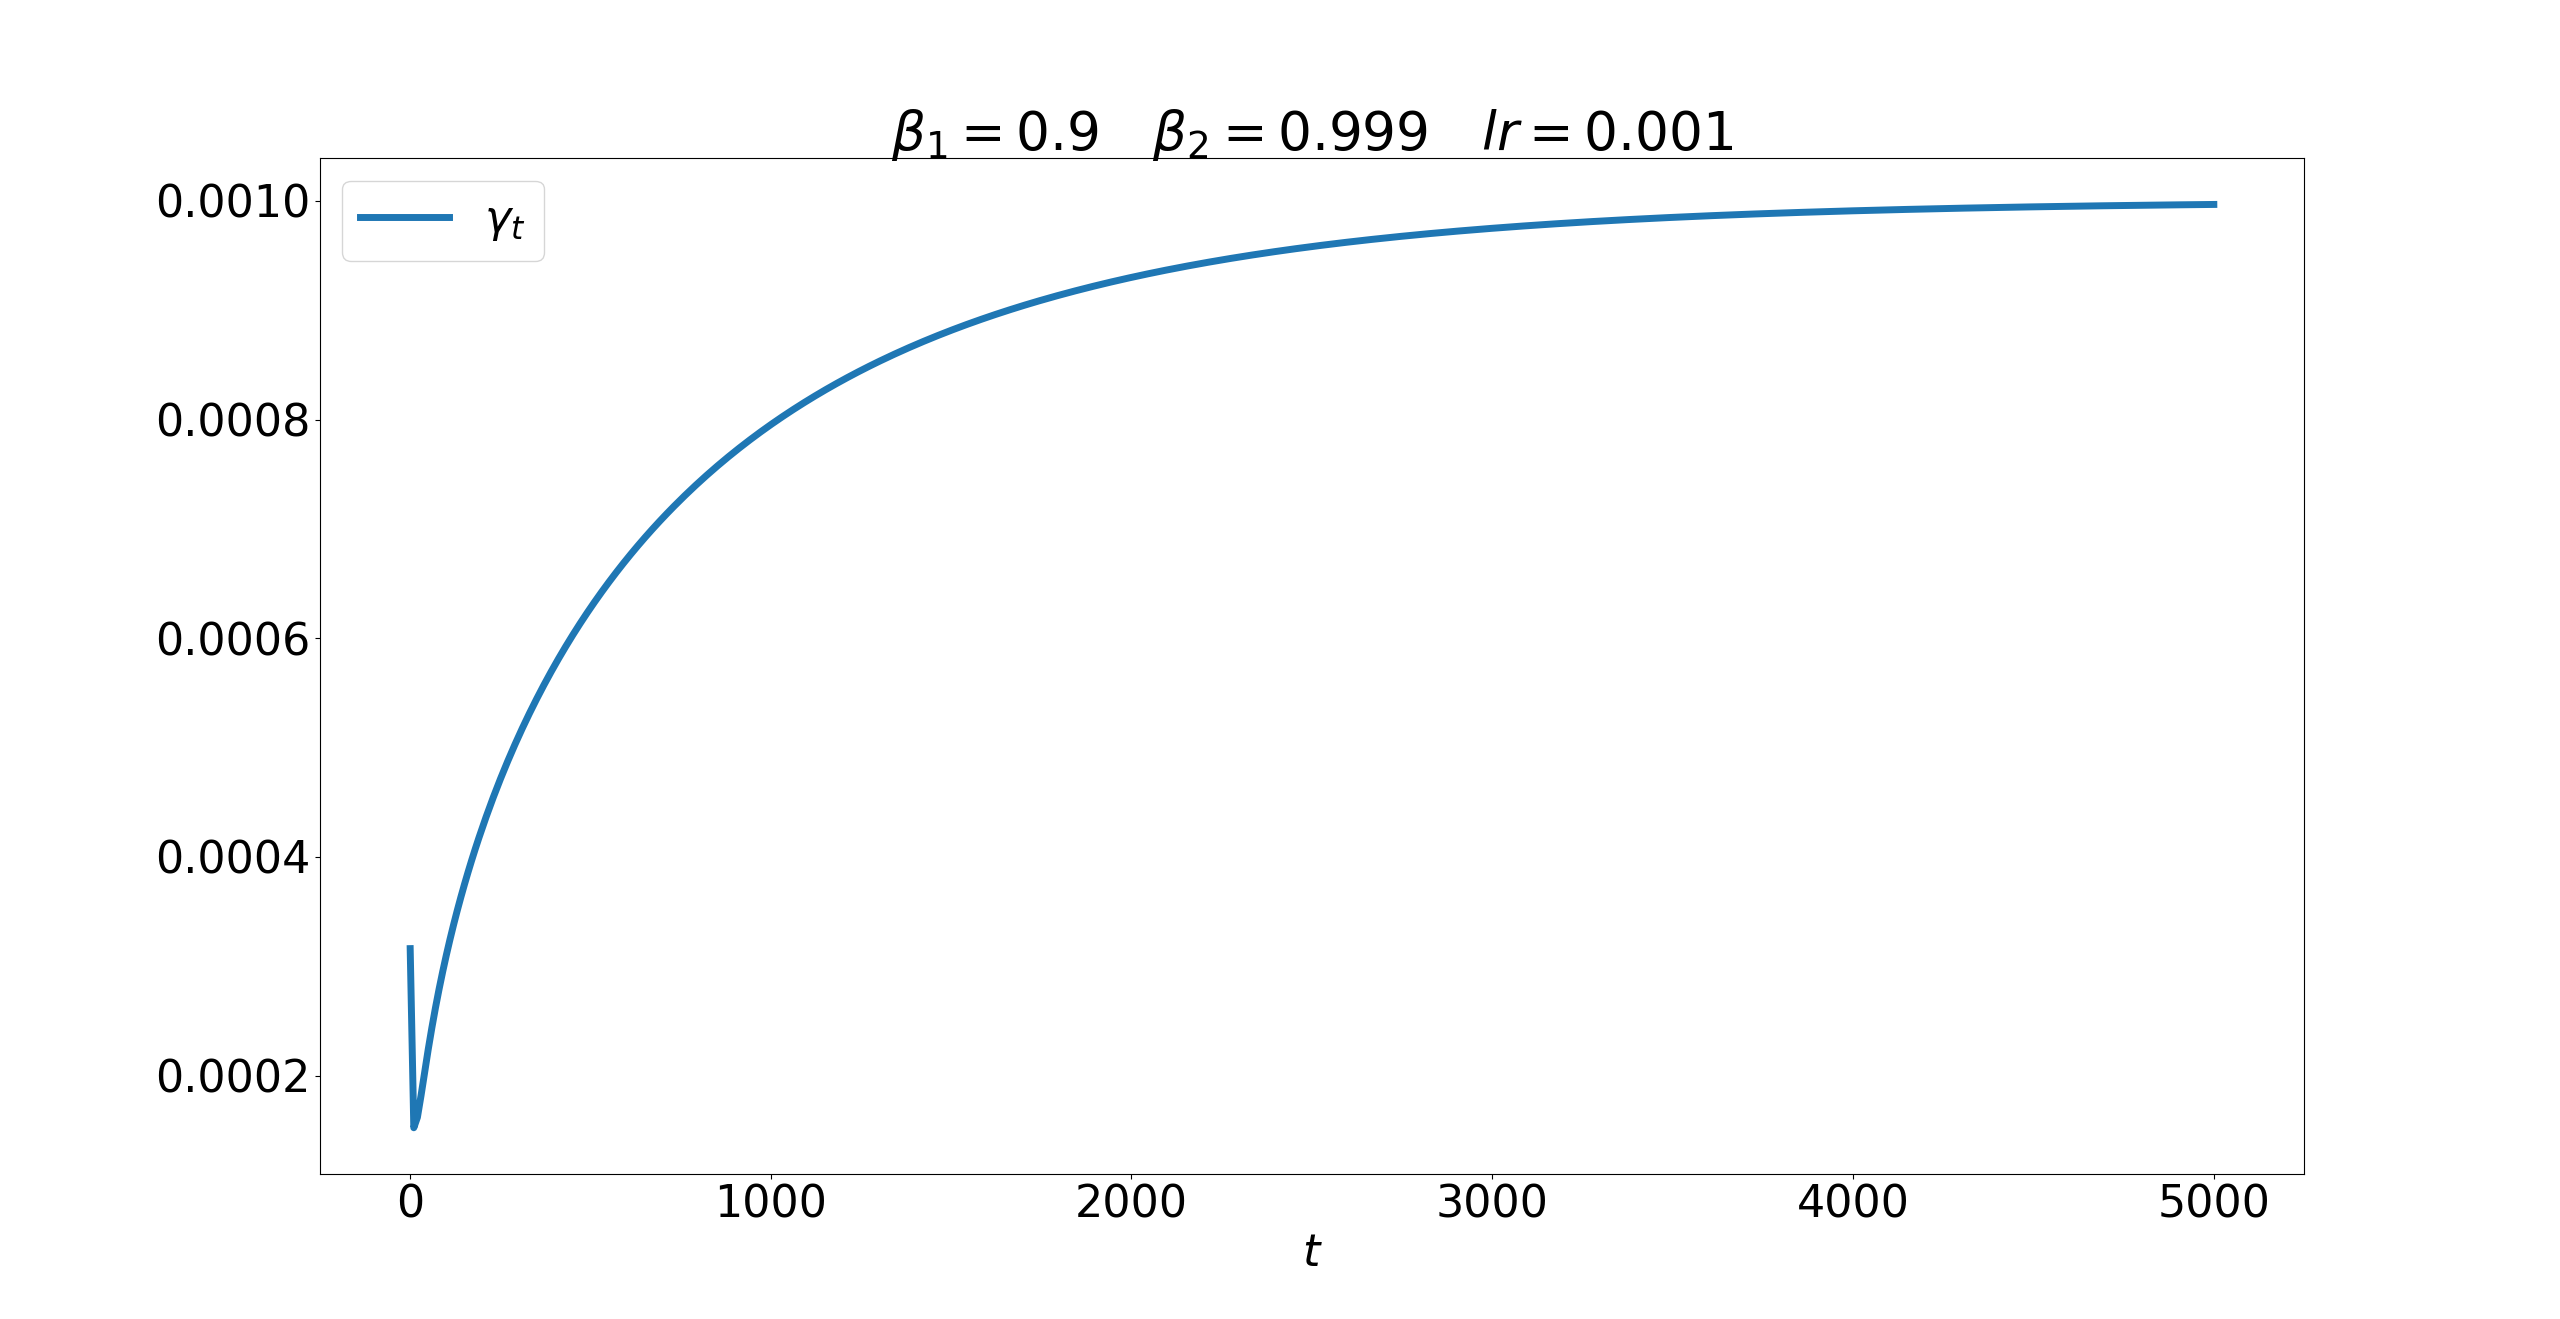
\includegraphics[width=0.8\linewidth]{images/adam.png}
		\caption{Adjusted learning rate (i.e. equation \eqref{adam:lr}) at beginning $5000$ steps}
	\end{figure}
\end{frame}

\subsection{AdaMax}
\begin{frame}
	\frametitle{AdaMax}
	\begin{itemize}
		\item {\bf AdaMax} generalize the $L_2$ norm of gradients of Adam in equation \eqref{adam:l2} to $p$ norm $L_p$.
		\item With some slight modification, we have
		\begin{align}\nonumber
			\bb v_t &= \beta_2^p\bb v_{t-1} + (1-\beta_2^p)\Vert\bb g_t\Vert^p \\
			&= (1-\beta_2^p)\sum_{i=1}^t\beta_2^{p(t-i)}\cdot\Vert\bb g_i\Vert^p.
		\end{align}
		Note that we replace $\beta_2$ with $\beta_2^p$.
	\end{itemize}

	\blfootnote{Kingma, Diederik P., and Jimmy Ba. 2014. “Adam: A Method for Stochastic Optimization.” ArXiv:1412.6980 [Cs], December. http://arxiv.org/abs/1412.6980.}
\end{frame}

\begin{frame}
	\frametitle{AdaMax}
	\begin{itemize}
		\item Let $p\rightarrow\infty$, then:
		\begin{align}\nonumber
			\bb u_t := \lim_{p\rightarrow\infty}(\bb v_t)^{1/p} &= \lim_{p\rightarrow\infty}\left((1-\beta_2^p)\sum_{i=1}^t\beta_2^{p(t-i)}\cdot\Vert\bb g_i\Vert^p\right)^{1/p} \\ \nonumber
			&= \lim_{p\rightarrow\infty}(1-\beta_2^p)^{1/p}\left(\sum_{i=1}^t\beta_2^{p(t-i)}\cdot\Vert\bb g_i\Vert^p\right)^{1/p} \\ \nonumber
			&= \lim_{p\rightarrow\infty}\left(\sum_{i=1}^t\left(\beta_2^{t-i}\cdot\Vert\bb g_i\Vert\right)^p\right)^{1/p} \\
			&= \max(\beta_2^{t-1}\Vert\bb g_1\Vert, \beta_2^{t-2}\Vert\bb g_2\Vert, \cdots, \beta_2\Vert\bb g_{t-1}\Vert, \Vert\bb g_t\Vert).
		\end{align}
		which can be write into a recursive formula:
		\begin{equation}
			\bb u_t = \max(\beta_2\cdot\bb u_{t-1}, \Vert\bb g_t\Vert)
		\end{equation}
		with initial value $\bb u_0 = \bb0$.
	\end{itemize}
\end{frame}

\begin{frame}
	\frametitle{AdaMax}
	\begin{itemize}
		\item Now we have AdaMax algorithm
		\vspace{2mm}
		\begin{formula}{AdaMax}
			\begin{align}
				\bb m_t &= \beta_1\bb m_{t-1}+(1-\beta_1)\nabla_{\bst}f(\bst_t) \\
				\bb u_t &= \max(\beta_2\cdot\bb u_{t-1}, \Vert\bb\nabla_{\bst}f(\bst)_t\Vert)  \\
				\bst_{t+1} &=\bst_t-\frac{\gamma}{(1-\beta_1^t)(\bb u_t + \epsilon)}\odot\bb m_t.
			\end{align}
		\end{formula}
	\end{itemize}
\end{frame}

\subsection{NAdam}
\begin{frame}
	\frametitle{Nesterov Adaptive Momeuntum, NAdam}
	\begin{itemize}
		\item We know that Adam $\approx$ Momentum $\oplus$ RMSProp and Nesterov is an improved version of Momentum. So we can replace Momentum with a modified version of Nesterov in Adam and get {\bf Nesterov Adam(NAdam)}.
		\item For Momentum update rule we can put them into one line:
		\begin{equation}
			\bst_{t+1}=\bst_t-(\beta\bb m_{t-1}+\gamma\nabla_{\bst}f(\bst_t)).
		\end{equation}
		\item And for Nesterov update rule:
		\begin{equation}
			\bst_{t+1}=\bst_t-(\beta\bb m_{t-1}+\gamma\nabla_{\bst}f(\bst_t-\beta\bb m_{t-1})).
		\end{equation}
		\item In NAdam, we replace $\bb m_{t-1}$ in Momentum with $\bb m_t$ directly, which can be viewed as a weighted momentum:
		\begin{equation}
			\bst_{t+1}=\bst_t-(\beta^2\bb m_{t-1} + (\beta+1)\gamma\nabla_{\bst}f(\bst_t)).
		\end{equation}
	\end{itemize}

	\blfootnote{Dozat, Timothy. 2016. “Incorporating Nesterov Momentum into Adam.”}
\end{frame}

\begin{frame}
	\frametitle{Nesterov Adaptive Momeuntum, NAdam}
	\begin{itemize}
		\item We can formalize Adam to a single line:
		\begin{equation}
			\bst_{t+1}=\bst_t-\frac{\gamma_t}{\sqrt{\bb v_t}+\epsilon}\odot(\beta_1\bb m_{t-1} + (1-\beta_1)\nabla_{\bst}f(\bst_t))
		\end{equation}
		Replace $\bb m_{t-1}$ with $\bb m_t$ and we get NAdam
		\begin{formula}{NAdam}
			\begin{align}
				\gamma_t &= \gamma\frac{\sqrt{1-\beta_2^t}}{1-\beta_1^t} \\
				\widetilde{\bb m}_t &= \beta_1\bb m_t + (1-\beta_1)\nabla_{\bst}f(\bst_t) \\
				\bb v_t &= \beta_2\bb v_{t-1}+(1-\beta_2)\nabla_{\bst}f(\bst_t)^2  \\
				\bst_{t+1} &=\bst_t-\frac{\gamma_t}{\sqrt{\bb v_t}+\epsilon}\odot\widetilde{\bb m}_t.
			\end{align}
		\end{formula}
	\end{itemize}
\end{frame}

{
	\setbeamertemplate{headline}{} 
	\begin{frame}
		\centering \Large
		  Thank You!
	\end{frame}
}
\addtocounter{framenumber}{-1}

\end{document}